%----------------------------------------------------------------------------------------
%	PACKAGES AND THEMES
%----------------------------------------------------------------------------------------
\documentclass[aspectratio=169,xcolor=dvipsnames,handout]{beamer}
\usetheme{SimplePlus}
\usepackage{fontawesome}
\usepackage{bm}

\usepackage{hyperref}
\usepackage{graphicx} % Allows including images
\graphicspath{ {../output/} }
\usepackage{booktabs} % Allows the use of \toprule, \midrule and \bottomrule in tables
\usepackage{subcaption}

\usepackage[style=ieee]{biblatex}
\setbeamertemplate{bibliography item}{\insertbiblabel}
\addbibresource{../report/bibliography.bib}

\usepackage{pgf-pie} % Allows creating pie charts

	
\usepackage{color, colortbl}


\usepackage{pgfplots} % Allows creating other plots
\pgfplotsset{compat=1.18}

\usepackage{caption}

\usepackage{pifont}

\usepackage{tikz} % Flow chart
\usetikzlibrary{shapes.geometric, arrows}
%----------------------------------------------------------------------------------------
%	TITLE PAGE
%----------------------------------------------------------------------------------------

\title[short title]{Heart Failure: predicting hospital re-admission after 6 months} % The short title appears at the bottom of every slide, the full title is only on the title page
\subtitle{Statistical Learning for Healthcare Data (056867) -- A.Y. 2022/2023}

\author[]{Teo Bucci, Giulia Montani and Alice Traversa}

\institute[] % Your institution as it will appear on the bottom of every slide, may be shorthand to save space
{
    
\includegraphics[width=3cm]{logo_polimi}%Politecnico di Milano% Your institution for the title page
}
\date{June 6, 2023} % Date, can be changed to a custom date


%----------------------------------------------------------------------------------------
%	PRESENTATION SLIDES
%----------------------------------------------------------------------------------------

\begin{document}

\begin{frame}
    % Print the title page as the first slide
    \titlepage
\end{frame}

% \begin{frame}{Overview}
%     % Throughout your presentation, if you choose to use \section{} and \subsection{} commands, these will automatically be printed on this slide as an overview of your presentation
%     \tableofcontents
% \end{frame}


% 10 minuti

% 1 - intro
% 2 - presentazione dei dati + data cleaning iniziale [*]
% 3 - NaN
% 4 - NaN + imputation
% 5 - outlier
% 6 - feature selection (variance based + correlation)
% 7 - Training conditions: Class imbalance, The CV approach was a StratifiedKFold with 5 folds, performance index AUC
% 8 - [RESULTS] TABLE 1 Interpretability vs complexity
% 9 - Random Forest TABLE 2 confusion matrix + performance (F1 recall, precision...)
% 10 - Explaining predictions with SHAP
% 11 - Logistic Regression: si allena velocemente, quindi feature selection scegliendo un numero di features guardando l'AUC al diminuire delle features
% 13 - limitations, further development and recommendations
% 
% 
% 
% [*] The majority of patients had age in the 59-89
% range, namely a total of 1680 patients accounting
% for 86.11% of the total. Regarding sex, 58.18% were
% females and 41.82% were males.
% 73.50% suffered a whole HF, while 23.89% suf-
% fered a Left HF and 2.61% a Right HF




%------------------------------------------------
\section{Introduction}
%------------------------------------------------



\begin{frame}{Problem statement}
    Heart failure (HF) is a prevalent condition with high re-admission rates.\\
    Number of HF cases worldwide:
    \begin{itemize}
        \item 33.5 million in 1990;
        \item 64.3 million in 2017.
    \end{itemize}
    
    \textbf{Half} of the patients diagnosed with HF will be re-admitted \textbf{once within a year} and 20\% will be re-admitted twice or more.
    \pause
    \begin{block}{Primary goal of the project}
        Develop a \textbf{prediction} model with focus on \textbf{interpretability}.
    \end{block}

    \begin{block}{Parallel objective}
        Assess the \textbf{importance of drugs} assumption.
    \end{block}

\end{frame}



%------------------------------------------------
\section{Materials and methods}
%------------------------------------------------

%------------------------------------------------

\begin{frame}{Data}
    \begin{columns}[t]
        \column{.7\textwidth}
        \begin{itemize}
            \item 2008 patients admitted to a hospital, of which were discarded:
            \begin{itemize}
                \item 57 dead patients
                \item 5 patients with inconsistent information
            \end{itemize}
            
            \item 168 variables provided, including:
            \begin{itemize}
                \item Demographic data (height, sex, occupation, \ldots).
                \item Medical history (diabetes, comorbidities, \ldots).
                \item Clinical measurements (pressure, hemoglobyn, \ldots).
                \item Drugs taken.
                \item Re-hospitalizations prior to 6 months (discarded).
            \end{itemize}
        \end{itemize}
        \pause

        \begin{figure}
        \centering

        \begin{minipage}{.3\textwidth}
            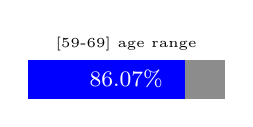
\begin{tikzpicture}
                \fill[Blue] (0,0) rectangle (2.5,0.5);
                \fill[Gray!90] (2.5,0) rectangle (2,0.5);
                \node at (1.25,0.25) [align=center] {\footnotesize \color{white}86.07\%};
                \node at (1.25,0.7) {\tiny [59-69] age range};
            \end{tikzpicture}
        \end{minipage}%
        \begin{minipage}{.3\textwidth}
            \resizebox{\textwidth}{!}{
            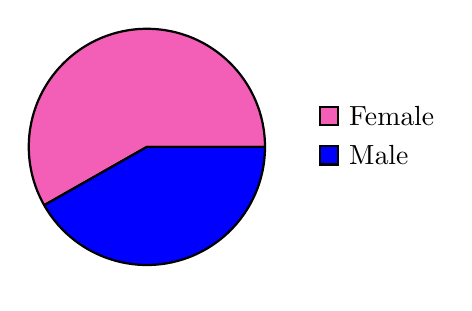
\begin{tikzpicture}
                \pie[
                    color={CarnationPink, Blue},
                    sum=auto,
                    text=legend,
                    before number=\phantom,,
                    radius=1.5
                ]{
                    58.22/Female,
                    41.78/Male
                }
            \end{tikzpicture}
            }
            %\caption{Distribution of Sex.}
        \end{minipage}%
        \begin{minipage}{.3\textwidth}
            \resizebox{\textwidth}{!}{
            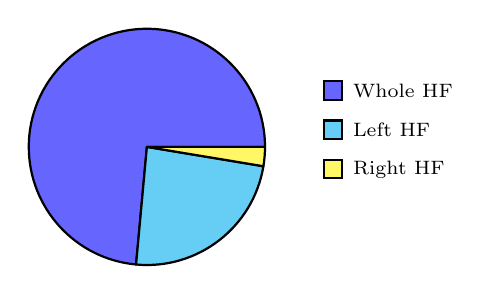
\begin{tikzpicture}[font=\scriptsize]
                \pie[
                    sum=auto,
                    text=legend,
                    before number=\phantom,,
                    radius=1.5
                ]{
                    73.54/Whole HF,
                    23.84/Left HF,
                    2.62/Right HF
                }
            \end{tikzpicture}
            }
            %\caption{Distribution of Heart Failure types.}
        \end{minipage}
        \end{figure}

        \column{.3\textwidth}
        \pause
        \begin{figure}[htpb]
            \centering
            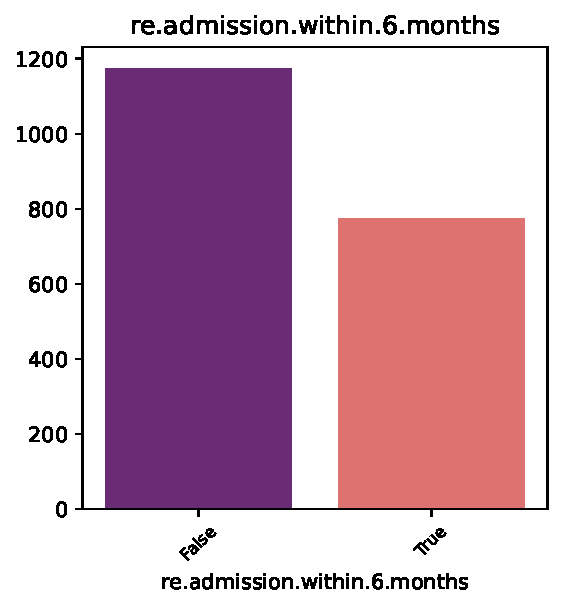
\includegraphics[width=\textwidth]{plot_target.pdf}
            \captionsetup{font=tiny} % Set the caption font size to small
            \caption{Target distribution.}
        \end{figure}
        

    \end{columns}
\end{frame}

% \begin{frame}{Pipeline}
% \begin{enumerate}
%     \item Data cleaning
%     \item Handle missing values
%     \item Dimensionality reduction
%     \begin{itemize}
%         \item Outlier analysis
%         \item Low variance variables
%         \item Correlation analysis
%     \end{itemize}
%     \item Feature selection
%     \item Model selection
%     \item Evaluation
% \end{enumerate}
% \end{frame}

%------------------------------------------------

\begin{frame}{Handling missing values}

    \begin{columns}[c]
        \column{.45\textwidth}
        \textbf{Categorical features}
        
        \begin{itemize}
            \item \texttt{Occupation} 1.34\%
            \item Imputation: most frequent
        \end{itemize}

        \vspace{0.5cm}
        \pause
        \textbf{Numerical features}

        \begin{itemize}
            \item 14 features with over 60\% missing are discarded
            \item 9 features between 50\% and 60\% are discarded after further analysis
            \item Imputation: KNN with 5 neighbors 
        \end{itemize}

        \column{.55\textwidth} 
        \begin{figure}[htpb]
            \centering
            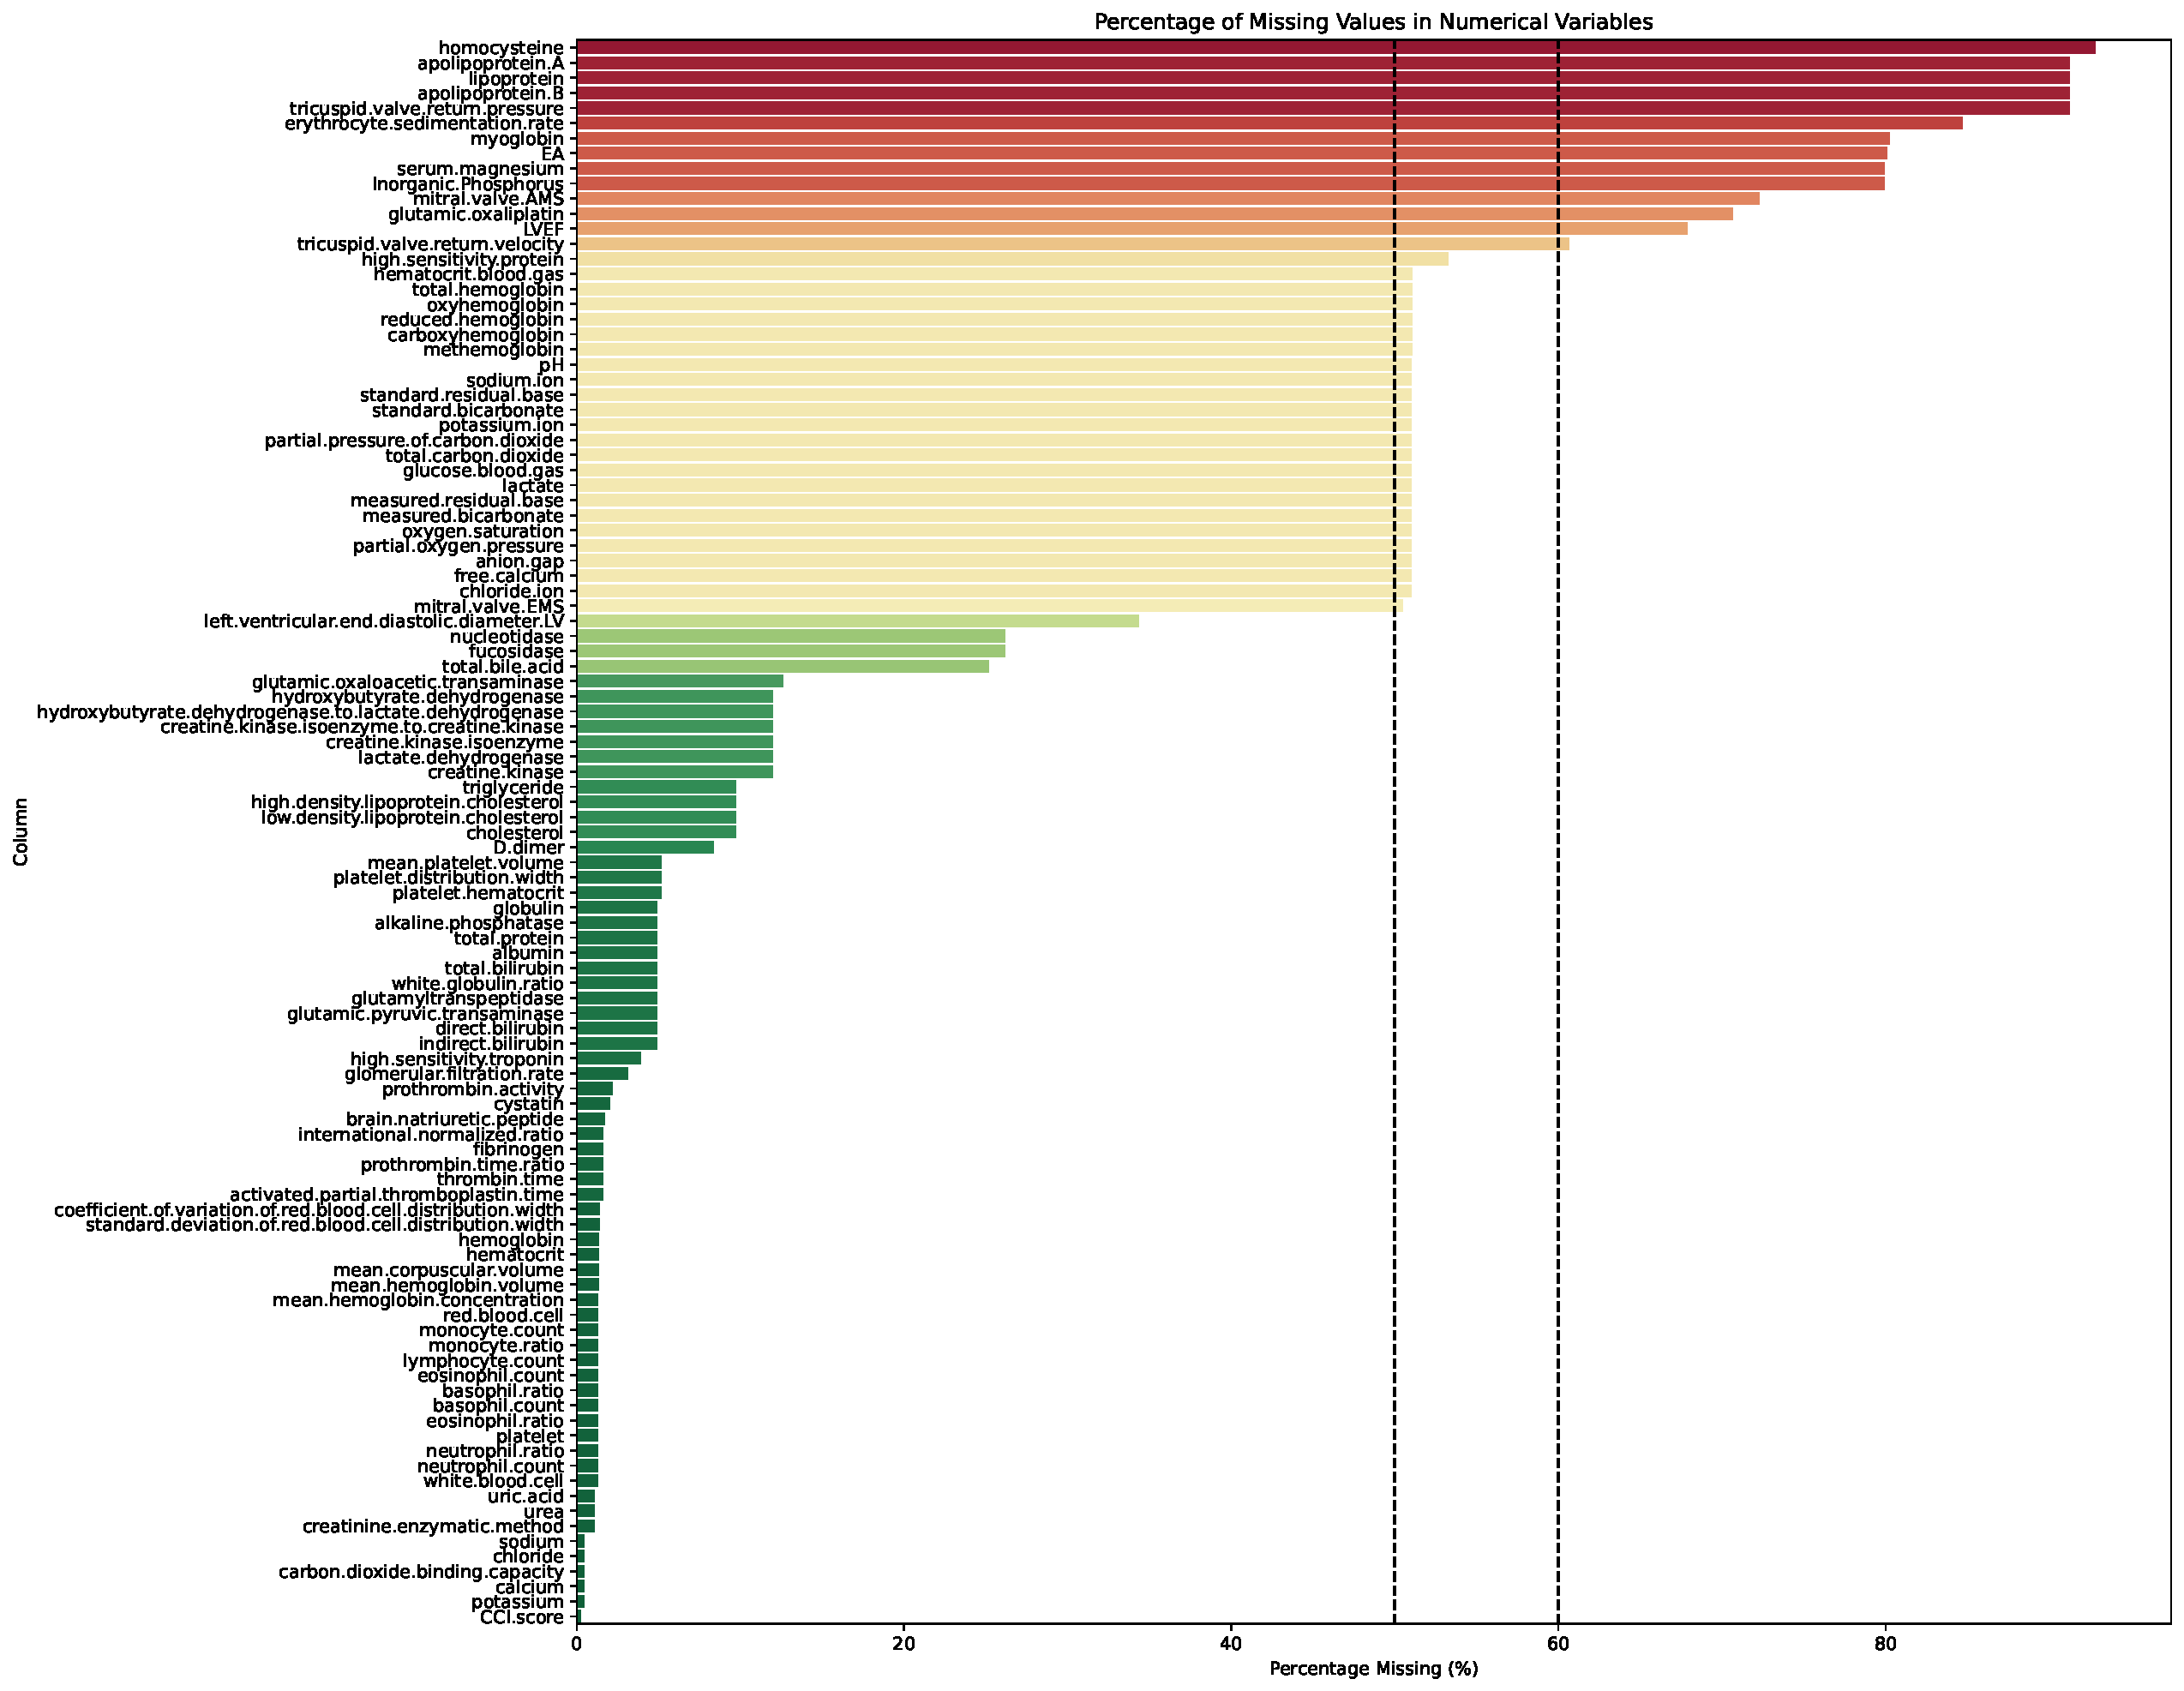
\includegraphics[width=0.9\textwidth]{missing_values_percentages.pdf}
            \captionsetup{font=tiny} % Set the caption font size to small
            \caption{Percentage of missing values in numeric.}
        \end{figure}
        
    \end{columns}

\end{frame}

%------------------------------------------------

\begin{frame}{Further cleaning}
\begin{itemize}
    \item \textbf{Outlier analysis}
    \begin{enumerate}
        \item Identification:
            \begin{itemize}
                \item Sample Z-scores.
                \item Physiological limits checked using literature.
            \end{itemize}
        \item Replace with \text{NaN} for imputation.
    \end{enumerate}
    \pause
    \item \textbf{Low variance variable:}
    Remove \alert{16} variables with more than \alert{95\% dominance}
    \pause
    \item \textbf{Correlation analysis:}
    Remove \alert{12} variables with more than \alert{85\% correlation}
\end{itemize}
\pause
Three variables with possible outliers retained due to their importance:
\begin{itemize}
    \item \texttt{eosinophil.count}
    \item \texttt{high.sensitivity.troponin}
    \item \texttt{glutamic.pyruvic.transaminase}
\end{itemize}

\end{frame}
%------------------------------------------------
\tikzstyle{method1} = [rectangle, rounded corners, 
minimum width=4cm, 
minimum height=1cm,
text width=4cm,
text centered, 
draw=black, 
fill=CornflowerBlue!70]

\tikzstyle{method2} = [rectangle, rounded corners, 
minimum width=4cm, 
minimum height=1cm,
text width=4cm,
text centered, 
draw=black, 
fill=Peach!70]

\tikzstyle{union1} = [rectangle, 
minimum width=1cm, 
minimum height = 0.5cm,
text centered, 
draw=black]

\tikzstyle{union2} = [rectangle, 
minimum width=1cm, 
minimum height = 0.5cm,
text centered, 
draw=Red]

\begin{frame}{Feature selection}

    \begin{figure}[!h]
    \centering
        \begin{tikzpicture}[node distance=2cm]
            \node (RF) [method1] {Random Forest
            \tiny{Set of 30 features: $S_{RF}$}};
            \node (LR) [method1, below of=RF] {Logistic Regression\\
            \tiny{Strong $L^{1}$ penalty: $S_{LR}$}};
            \node (U1) [union1, right of = LR, yshift= 1cm, xshift = 1cm] {\tiny{$S_{RF}\cup S_{LR}$}};
            \node (BS) [method2, right of = U1, yshift = 1cm, xshift = 1cm] {Backward
            \\ \tiny{Elbow threshold: $S^{\star}_{1}$}};
            \node (FS) [method2, right of = U1, yshift = -1cm, xshift = 1cm] {Forward 
            \\ \tiny{Elbow threshold: $S^{\star}_{2}$ }};
            \node (U2) [union2, right of = FS, yshift= 1cm, xshift = 2cm] {\tiny{$S = S^{\star}_{1}\cup S^{\star}_{2}$}};
    
            \draw [->] (RF) -- (U1);
            \draw [->] (LR) -- (U1);
            \draw [->] (U1) -- (BS);
            \draw [->] (U1) -- (FS);
            \draw [->] (FS) -- (U2);
            \draw [->] (BS) -- (U2);
            
        \end{tikzpicture}
    \end{figure}

    %\vspace{5cm}
    
    %\textbf{Strength of the method:} 
    %\begin{itemize}
    %    \item Faster than backward selection
    %    \item Take advantages of both RF and LR
    %    \item Final set of 13 selected variables.
    %\end{itemize}
    \pause
    \begin{block}{Strength of the method}
    \begin{itemize}
        \item Faster than performing backward selection immediately.
        \item Takes away a lot of the \emph{greedyness}.
        \item Takes advantages of both RF and LR (intersection is very small).
    \end{itemize}
    \end{block}
    Final set of 13 selected variables.

    
\end{frame}

%------------------------------------------------
\begin{frame}{Model selection}

Train 6 different classifiers.

\pause
\textbf{Metric}
\begin{itemize}
    \item Compare performance between models using \textbf{AUC}.
\end{itemize}

\pause
\textbf{Training setting} 
\begin{itemize}
    \item Preprocessing: one-hot encoding and scaling.
    \item \textbf{Tune hyperparameters} with GridSearchCV.
    \item Evaluate performance using \textbf{Stratified 5-fold} cross-validation (CV).
    \item 85:15 stratified train-test ratio.
    \item Always set seed for reproducibility.
    \item Class imbalance addressed by passing class weights based on sample proportions.
\end{itemize}
    
\end{frame}


%------------------------------------------------
\section{Results}
%------------------------------------------------



%------------------------------------------------

\begin{frame}{Results}

    \begin{columns}[c]
        \column{.5\textwidth}
        \begin{table}[htpb]
        \centering
        %\caption{Comparison of performance.}
        \label{tab:performance}
        \begin{tabular}{lr}
        \toprule
                         Model &    AUC \\
        \midrule
        RandomForestClassifier & 0.6769 \\
        \rowcolor{green!50}
            LogisticRegression & 0.6702 \\
                    GaussianNB & 0.6452 \\
        DecisionTreeClassifier & 0.5943 \\
          KNeighborsClassifier & 0.5681 \\
                 MLPClassifier & 0.5028 \\
        \bottomrule
        \end{tabular}
        \caption{Comparison of performance.}
        \end{table}

        \column{.5\textwidth}
        \begin{figure}[htpb]
            \centering
            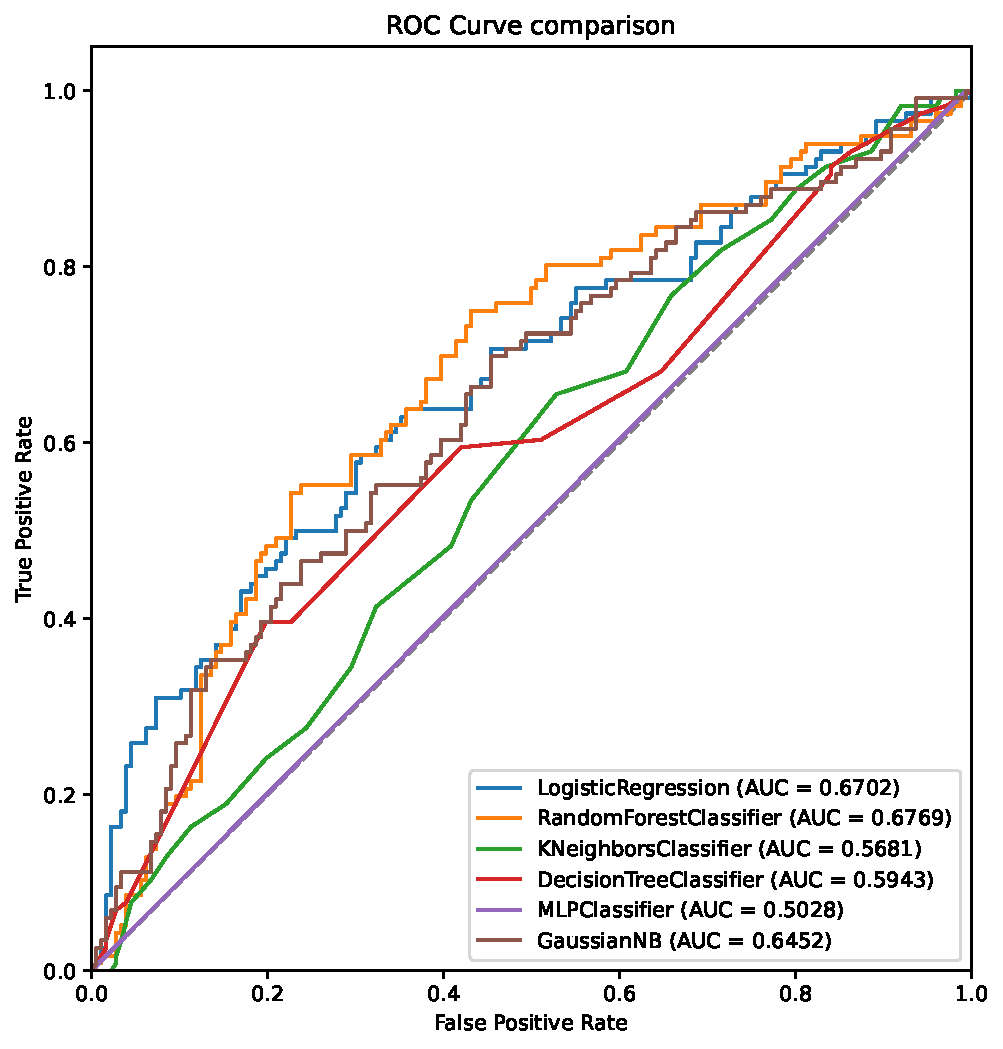
\includegraphics[width=2.1in]{roc_comparison.pdf}
            \caption{ROC curves comparison.}
            \label{fig:roc-comparison}
        \end{figure}
    \end{columns}

\end{frame}


% \begin{frame}{Results (cont.)}

% \begin{figure}[htpb]
%             \centering
%             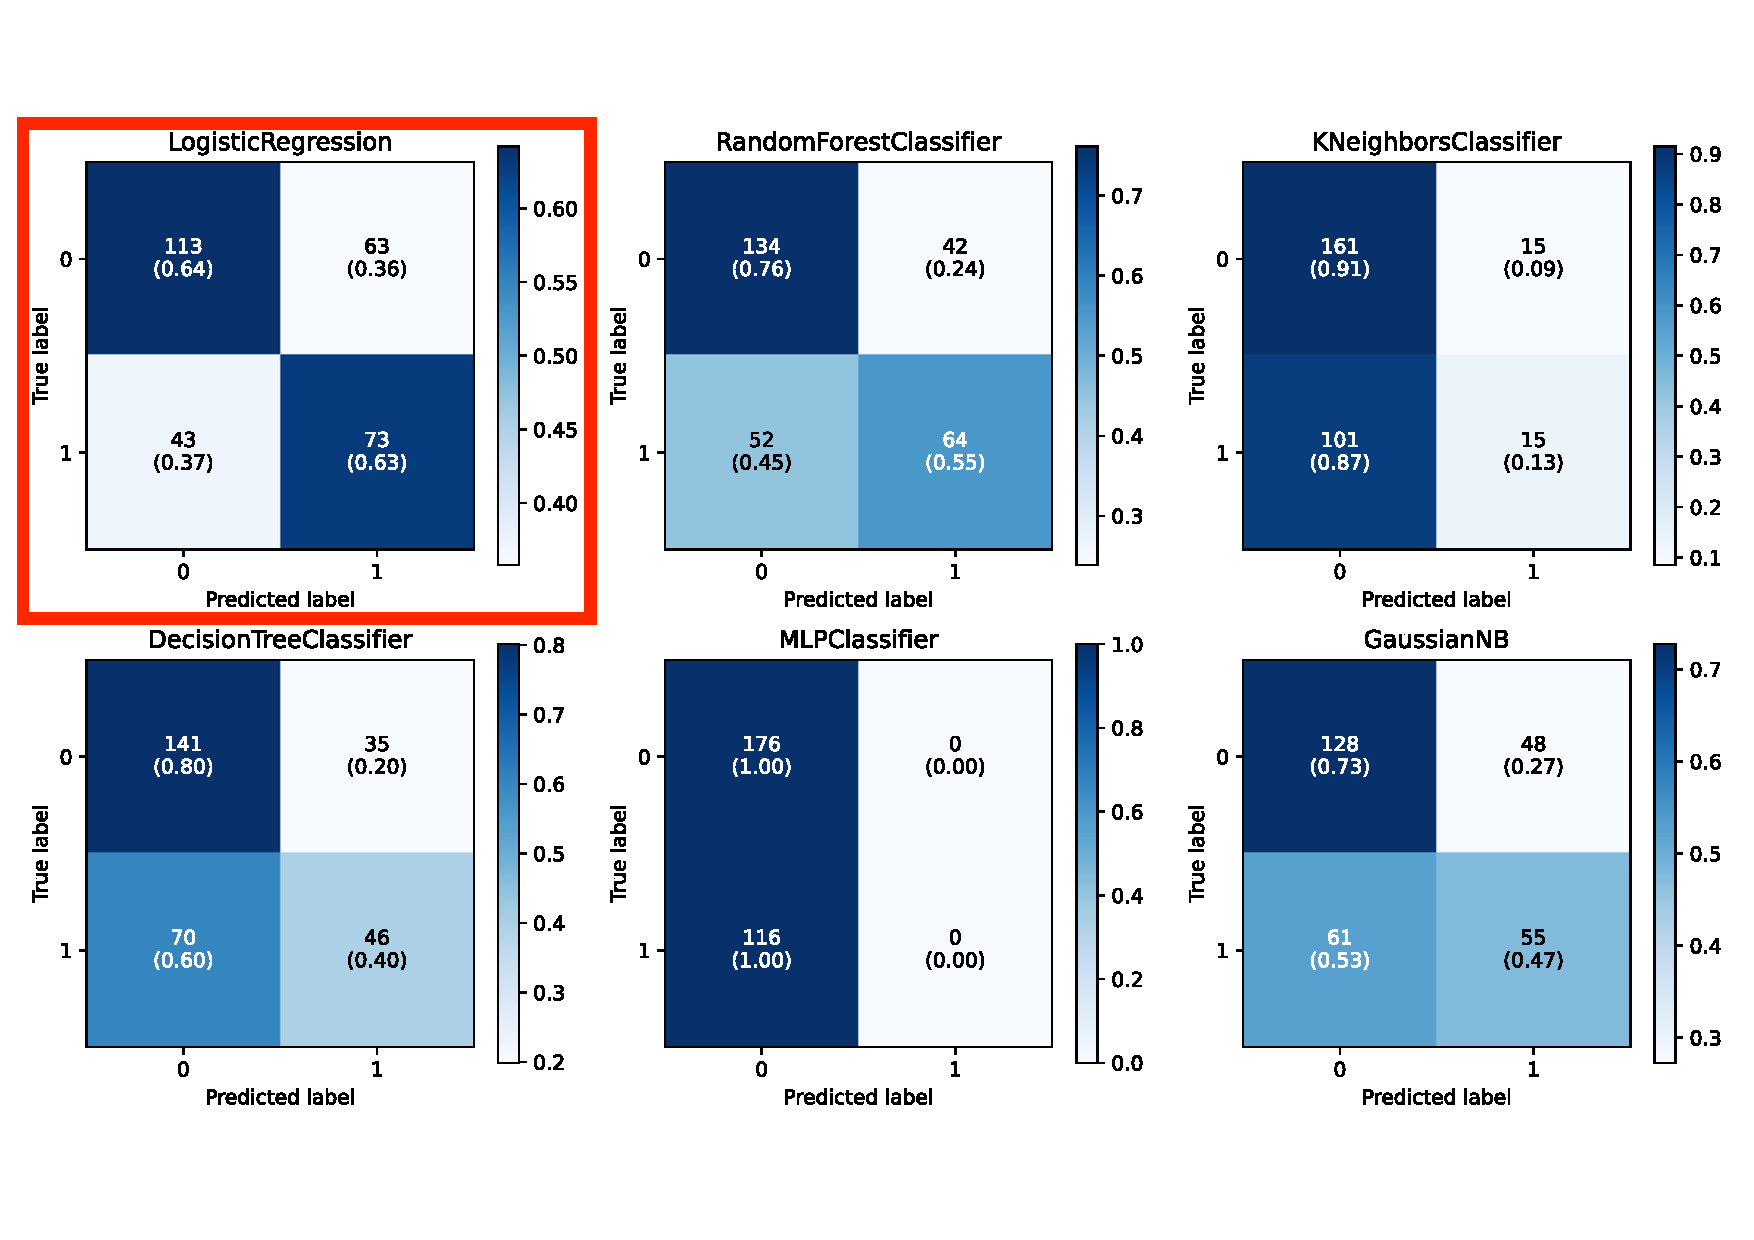
\includegraphics[width=0.7\textwidth]{confusion_matrices_annot}
%             \caption{Confusion matrices comparison (threshold: 0.5).}
%         \end{figure}

% \end{frame}

%------------------------------------------------

\begin{frame}{Results (cont.)}

    \begin{columns}[c]

        \column{.6\textwidth}
        \begin{figure}[htpb]
            \centering
            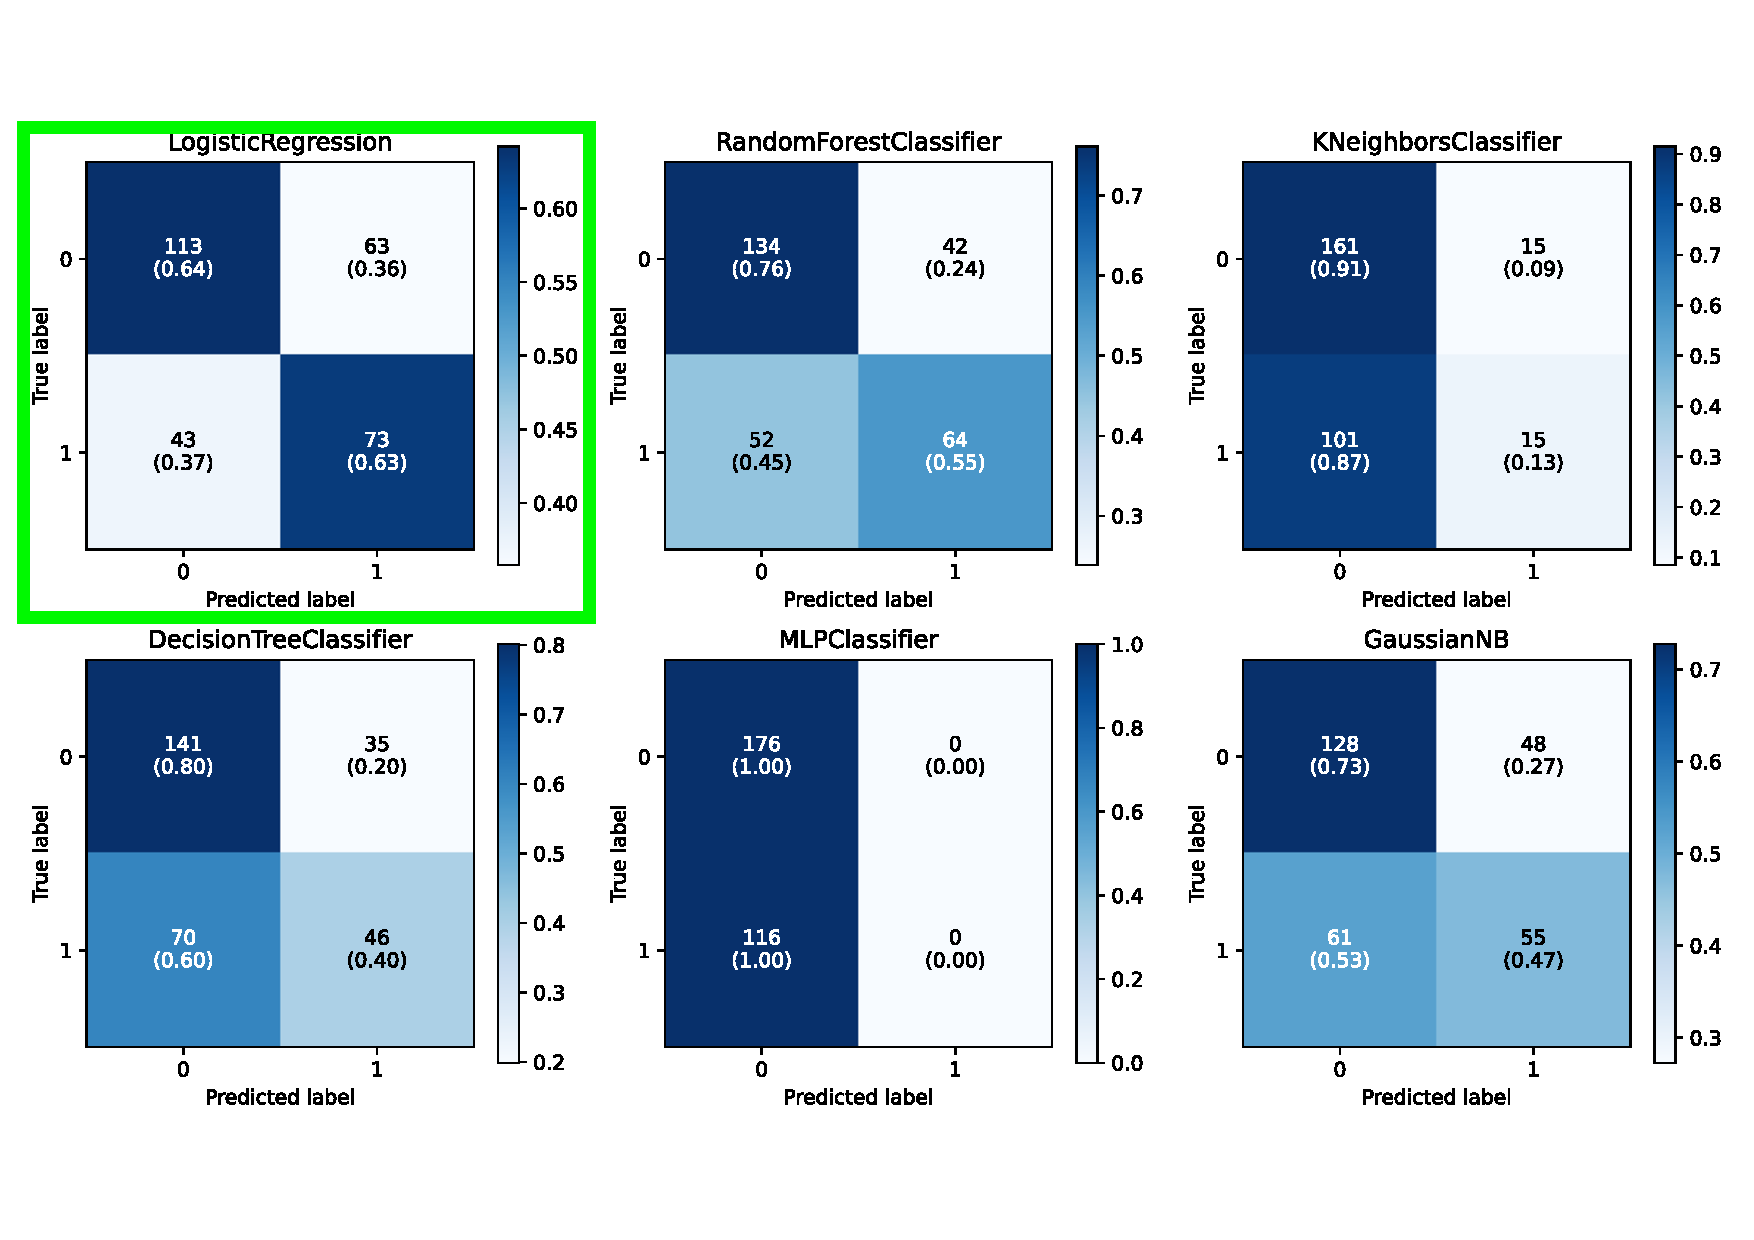
\includegraphics[width=\textwidth]{confusion_matrices_annot_green}
            \caption{Confusion matrices comparison (threshold: 0.5).}
        \end{figure}
        
% \vspace*{0.5cm}
% \textbf{Interpretation} of the model:
% \begin{align*}
% \operatorname{OR}_i &= \frac{\operatorname{odds}(\bm{X}+\bm{1}_i)}{\operatorname{odds}(\bm{X})} = \cdots = e^{\beta_i}
% \end{align*}
% The odds multiply by $e^{\beta_i}$ for every 1-unit increase in $X_i$.
    
        \column{.4\textwidth}
        Logistic Regression performance:
        \begin{itemize}
            \item AUC: \textbf{0.6702}
            \item Accuracy: \textbf{0.6370}
            \item Precision: 0.5368
            \item Recall: 0.6293
            \item F1-score: 0.5794
        \end{itemize}
        


        % \begin{figure}[htpb]
        %     \centering
        %     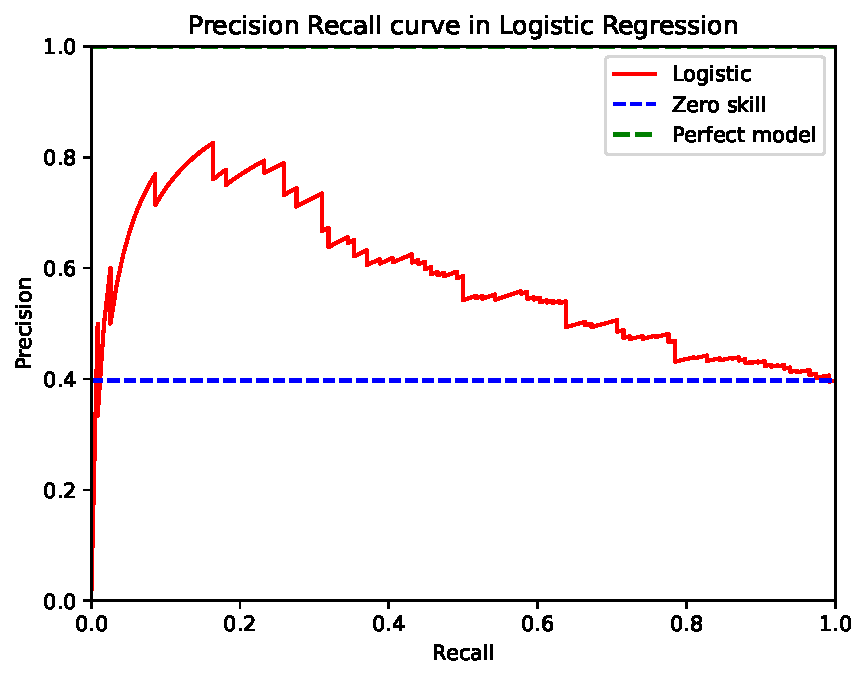
\includegraphics[width=\textwidth]{precision_recall_curve_LR}
        %     \caption{LR Precision-Recall curve.}
        % \end{figure}


        % \begin{figure}[htpb]
        %     \centering
        %     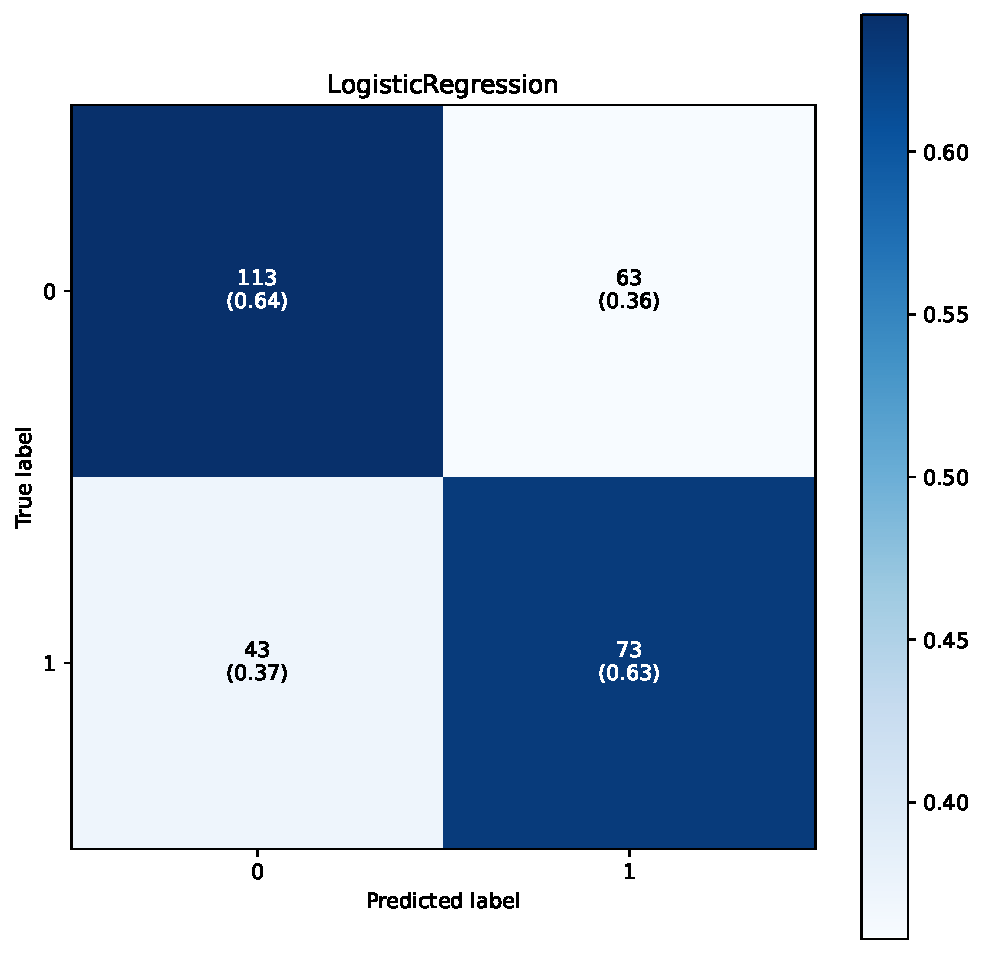
\includegraphics[width=\textwidth]{confusion_matrix_LR.pdf}
        %     \caption{Normalized confusion matrix.}
        % \end{figure}


        % \begin{table}
        %     \resizebox{0.8\textwidth}{!}{
        %     \begin{tabular}{lrrrr}
        %     \toprule
        %     Accuracy &  Precision &  Recall &  F1-score \\
        %     \midrule
        %     0.6370         &     0.5368 &  0.6293 &    0.5794\\
        %     \bottomrule
        %     \end{tabular}
        %     }
        %     \caption{Classification report.}
        % \end{table}
        
    \end{columns}
\end{frame}

%------------------------------------------------
\section{Conclusions}
%------------------------------------------------


%------------------------------------------------
\begin{frame}{Conclusions}

    \begin{columns}[c]

        \column{.5\textwidth}
        %\centering
        %\begin{figure}[htpb]
        %    \centering
        %    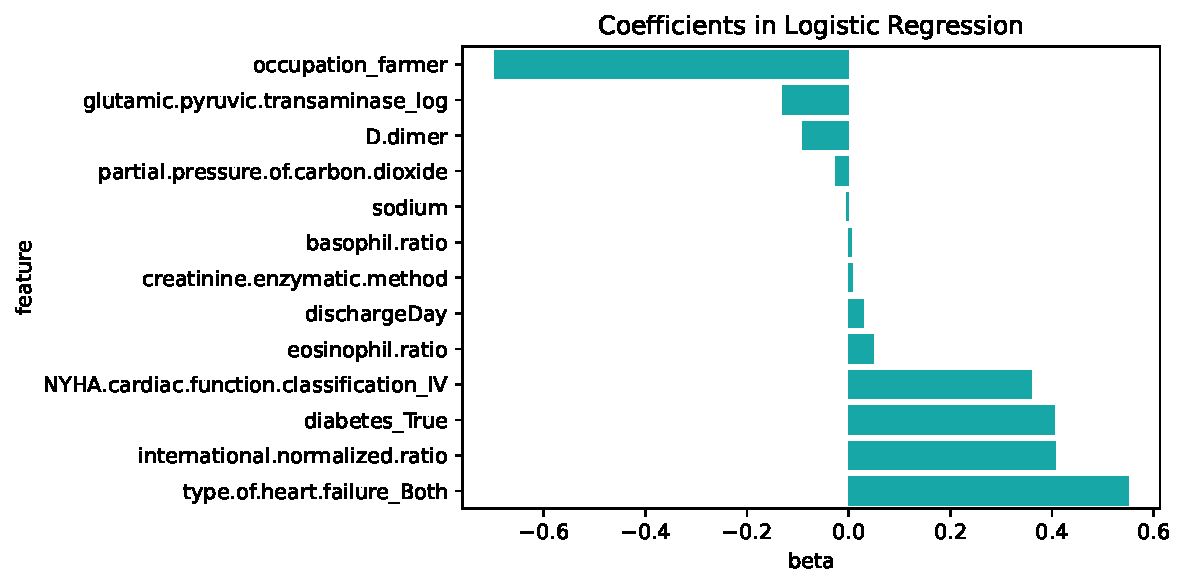
\includegraphics[width=2.6in]{feature_importance_weightsLogisticRegression.pdf}
        %    %\caption{Coefficients of the \gls{lr}.}
        %    \label{fig:feature-importance-logistic-regression}
        %\end{figure}

        \begin{table}[h!]
            \centering
        \resizebox{\textwidth}{!}{
        \begin{tabular}{lrr}
            \toprule
                                            feature &    beta &  exp\_beta \\
            \midrule
\rowcolor{cyan!50}
                                  occupation\_farmer & -0.6973 &    0.4979 \\
                  glutamic.pyruvic.transaminase\_log & -0.1305 &    0.8776 \\
\rowcolor{cyan!50}
                                            D.dimer & -0.0911 &    0.9129 \\
                 partial.pressure.of.carbon.dioxide & -0.0261 &    0.9743 \\
                                             sodium & -0.0049 &    0.9951 \\
                                     basophil.ratio &  0.0055 &    1.0055 \\
                        creatinine.enzymatic.method &  0.0066 &    1.0066 \\
\rowcolor{red!50}
                                       dischargeDay &  0.0294 &    1.0298 \\
                                   eosinophil.ratio &  0.0486 &    1.0498 \\
\rowcolor{red!50}
            NYHA.cardiac.function.classification\_IV &  0.3599 &    1.4332 \\
\rowcolor{red!50}
                                      diabetes\_True &  0.4049 &    1.4991 \\
                     international.normalized.ratio &  0.4074 &    1.5029 \\
\rowcolor{red!50}
                         type.of.heart.failure\_Both &  0.5502 &    1.7336 \\
            \bottomrule
            \end{tabular}
        }
            \caption{LR coefficients.}
        \end{table}

        \column{.5\textwidth}
        We found meaningful \textbf{interpretations} with clinical facts:
        \begin{itemize}
            \item \textbf{Farmers} are less likely to be re-admitted (probably external confounder).
            \item \textbf{D-dimer} seems associated with tissue repair.
            \item Higher \textbf{discharge day} (i.e. longer stay in hospital) is associated with higher risk.
            \item \textbf{Level 4 NYHA}, presence of \textbf{diabetes} and having suffered a \textbf{Whole HF} highly associated with re-admission.
        \end{itemize}
    \end{columns}
    
\end{frame}

\begin{frame}{Conclusions (cont.)}

    Regarding \textbf{drugs}, they were divided into 4 categories:
    \begin{itemize}
        \item Diuretics
        \item Vasodilatory
        \item Inhibitor
        \item Increase force of heart contraction (IFHC)
    \end{itemize}
    \pause
    Takeaways:
    \begin{itemize}
        \item None made it to the final set of features, so their importance is \textbf{not fundamental}.
        \pause
        \item \textbf{Most patients} are treated with both \textbf{diuretics and vasodilators}, therefore they don't help separation.
        \pause
        \item \textbf{IFHC} made it to the second step of feature selection, so it's the most informative category.
    \end{itemize}

\end{frame}


\begin{frame}{Deployment}
    \textbf{Web app} for easy usage by clinicians:
    {\scriptsize\url{https://teobucci-slhd-app-3iahgf.streamlit.app/}}
    \begin{figure}[htpb]
        \centering
        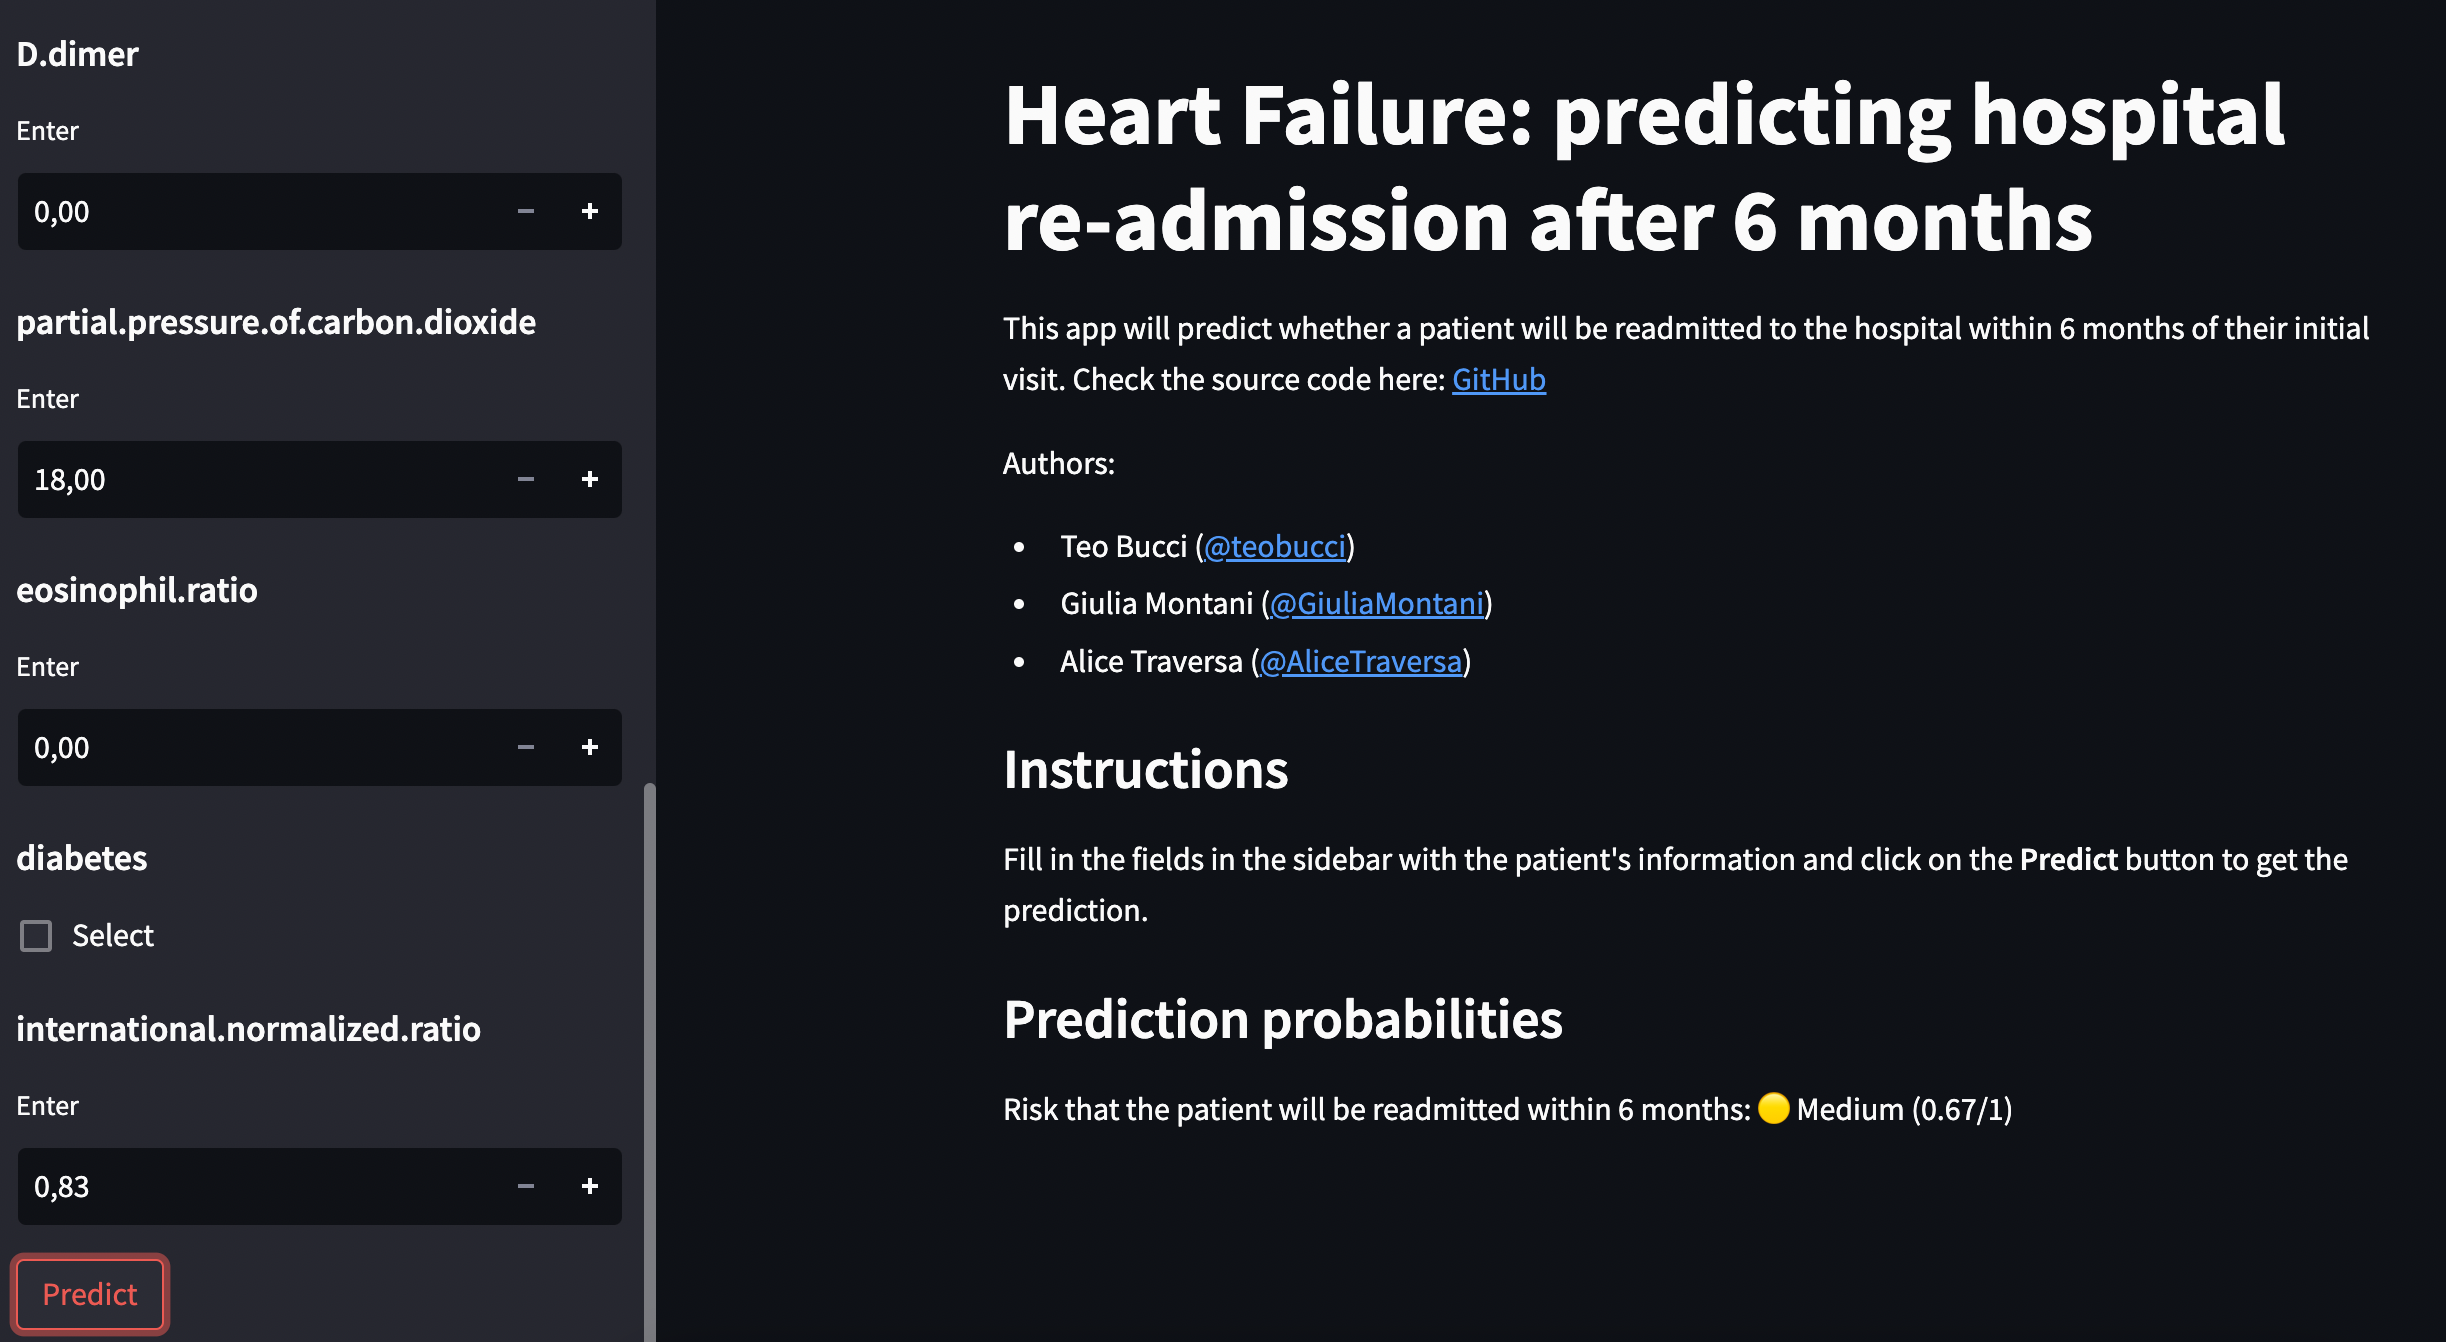
\includegraphics[width=0.7\textwidth]{webapp}
    \end{figure}
\end{frame}



% \begin{frame}{Limitations and Recommendations}
% \begin{itemize}
%   \item Limitations: reliance on \textbf{single dataset} and difficulty in \textbf{comparing results}, sample is \textbf{not representative}, missing data imputation, lacking data coming from electrocardiography.
%   \item Recommendations: better \textbf{management of missing values}, further validation with \textbf{external datasets}, exploration of \textbf{additional predictive models}.
% \end{itemize}
% \end{frame}
\begin{frame}{Limitations and Recommendations}
\textbf{Limitations}
\begin{itemize}
  \item reliance on \textbf{single dataset}
  \item difficulty in \textbf{comparing results}
  \item the sample is \textbf{not representative}
  \item missing data imputation
  \item lacking data coming from electrocardiography.
\end{itemize}
\pause
\textbf{Recommendations}
\begin{itemize}
  \item better \textbf{management of missing values} in the data
  \item further validation with \textbf{external datasets}
  \item for the sake of \textbf{performance} only, keep more variables and explore more models, at the cost of simplicity
\end{itemize}
\end{frame}






% \begin{frame}[fragile] % Need to use the fragile option when verbatim is used in the slide
%     \frametitle{Citation}
%     An example of the \verb|\cite| command to cite within the presentation:\\~

%     This statement requires citation \cite{p1}.
% \end{frame}

%------------------------------------------------

\begin{frame}
    \Huge{\centerline{\textbf{Thank You!}}}
    \begin{center}
    {\normalsize
    \faGithub\ \url{https://github.com/teobucci/slhd}}    
    \end{center}
\end{frame}

% %------------------------------------------------

\begin{frame}{References}
    \nocite{Bragazzi2021Burden}
    \nocite{Groenewegen2020Epidemiology}
    \nocite{Zhang2021Electronic}
    \nocite{Lonn2000Regular}
    \printbibliography
\end{frame}



%----------------------------------------------------------------------------------------

\end{document}